\documentclass{chi2009}
\usepackage{times}
\usepackage{url}
\usepackage{graphics}
\usepackage{color}
\usepackage[pdftex]{hyperref}
\hypersetup{%
pdftitle={CourseRatings: A Better Course Evaluation Catalog},
pdfauthor={Ryan Drapeau, Emily Gu, Vimala Jampala},
pdfkeywords={D3, React, JavaScript, Python, database, course evaluations},
bookmarksnumbered,
pdfstartview={FitH},
colorlinks,
citecolor=black,
filecolor=black,
linkcolor=black,
urlcolor=black,
breaklinks=true,
}
\newcommand{\comment}[1]{}
\definecolor{Orange}{rgb}{1,0.5,0}
\newcommand{\todo}[1]{\textsf{\textbf{\textcolor{Orange}{[[#1]]}}}}

\pagenumbering{arabic}  % Arabic page numbers for submission.  Remove this line to eliminate page numbers for the camera ready copy

\begin{document}
% to make various LaTeX processors do the right thing with page size
\special{papersize=8.5in,11in}
\setlength{\paperheight}{11in}
\setlength{\paperwidth}{8.5in}
\setlength{\pdfpageheight}{\paperheight}
\setlength{\pdfpagewidth}{\paperwidth}

% use this command to override the default ACM copyright statement
% (e.g. for preprints). Remove for camera ready copy.
\toappear{Submitted to CSE 512 (Spring) as the final paper.}

\title{CourseRatings: A Better Course Evaluation Catalog}
\numberofauthors{3}
\author{
  \alignauthor Ryan Drapeau\\
    \affaddr{University of Washington}\\
    \email{drapeau@\footnotemark[1]}
  \alignauthor Emily Gu\\
    \affaddr{University of Washington}\\
    \email{emilygu@\footnotemark[1]}
  \alignauthor Vimala Jampala\\
    \affaddr{University of Washington}\\
    \email{vjampala@\thanks{@cs.washington.edu}}
}

\maketitle

\begin{abstract}
Students at the University of Washington have very few resources to learn about what the classes they could sign up for are like. The University of Washington does provide a course evaluation catalog that summarizes student evaluations of courses. However, the catalog is difficult to use, with users having to rely on their browser's find functionality to search for courses. Additionally, the catalog only lists data from the previous two quarters, making it difficult to observe trends over time. In order to make this data easier to view and understand, we built CourseRatings, an online tool that provides displays evaluations of courses at the University of Washington. Built using React, D3, jQuery, Python, and TaffyDB, CourseRatings allows users to search for, sort through, visualize and compare courses they're interested in. CourseRatings has two goals - to give students and instructors access to the data they need to make informed choices about the classes they take or teach, as well as to present this data in an intuitive and user-friendly way.
\end{abstract}

\keywords{D3, React, JavaScript, Python, database, course evaluations}

\section{Introduction}

One of the most stressful times during the school year for a student is registration for the next quarter.  Picking the best classes and more importantly, the best instructor for the class could change a student's experience of a course. At the University of Washington (UW), students fill out an evaluation form for the instructors and courses as a whole at the end of each quarter.  Currently, UW releases this information in the Course Evaluation Catalog\footnote{\href{www.washington.edu/cec/}{www.washington.edu/cec/}} (CEC) to aid students in their search for classes \cite{cec}.

\subsection{Motivation}
Although the goal behind the catalog is helpful to students, the design of the page and the visualization of the data is not.  To find a specific course evaluation, students must first scroll through thousands of previous courses simply listed in alphabetical order.  With no search functionality, students resort to using the browser's find functionality which yields poor results much of the time.  After clicking on one of the courses, the user is presented with the evaluation data in a simple table.  Additionally, since the initial page consists of only a list of evaluations, comparing between different courses becomes a difficult task.

Not only is the design unintuitive, but the data presented conveys little information across to those using the site. When information on a particular class is displayed, all that is shown is the percentage of students that rated the professor ``Excellent'', ``Very Good'', ``Good'', ``Fair'', ``Poor'', and ``Very Poor'' on a particular dimension. It is not immediately obvious whether these ratings mean a class is rated highly or not.  The little information that can be gained by looking at this data takes much longer to understand than it should.  The site does not directly elicit any average or aggregate information about courses or professors, making it difficult to gain a ``big picture'' view of the class or any instructor. Additionally, with only the past two to three quarters of evaluation data shown on the UW Course Evaluation Catalog, any data before that time is lost to students.

As a result, we aimed to create a tool that would be useful to students and instructors alike to look at evaluations.  Such a tool would give students the ability to create a schedule with classes more suited for them, while also giving instructors the ability to easily understand the feedback they received. Our application reveals deeper insights and user friendly visualizations that would be useful when deciding what courses to take or which instructor to take a course from.

\section{Related Work}

There are several existing tools that are similar to CourseRatings at several noteworthy universities, though none of them sets out to achieve the same goals CourseRatings does.

The first is the University of Washington Course Evaluation Catalog, which has been outlined in the previous section in detail.

The second is BerkeleyTime\footnote{\href{www.berkeleytime.com/}{www.berkeleytime.com/}}, an online course catalog for the University of California, Berkeley \cite{berkeleytime}. The catalog has three main pages.  The first is a page to search for different courses offered where a course can be clicked to show information about that specific course. The second page is a comparison of grade distributions where the user can choose different courses to compare the grades received. For visuals, a bar chart is used while detailed information, for example average grade is listed. The last page is an enrollment breakdown page.  Different courses can also be added to the page and a line chart is used to show the data.

The Berkeley page strives to show a different set of data from what we do.  With data on grade distributions and more specific data than we do on enrollment, BerkeleyTime achieves the goal of making course selection simpler in a different manner than UW does. UW on the other hand, uses data from evaluations from students.

The third website is RateMyProfessors\footnote{\href{www.ratemyprofessors.com}{www.ratemyprofessors.com}}, which is a website that allows students to rate their professors and their university \cite{ratemyprofessors}. This website is similar to CourseRatings, in that it uses student ratings to help other students decide whether or not to take a class. Additionally, unlike CourseRatings, RateMyProfessors also displays comments from students, which provides additional context for the ratings. However, unlike CourseRatings, RateMyProfessors has few ratings per instructor and doesn't support a course search feature. The site is largely focused around providing a means to look up what students are saying about a particular professor. These ratings are also prone to selection bias, since the students who leave reviews on RateMyProfessors are students that have strong opinions about a particular instructor.

The final tool is MyEdu\footnote{\href{www.myedu.com}{www.myedu.com}}, a website targeted towards students and employers \cite{myedu}. MyEdu allows students to plan their schedules by selecting the courses they are registered for and specifying recurring events (such as work or group meetings). It also lets students browse courses and instructors. Like BerkeleyTime, clicking on a course page in MyEdu shows the average grade distribution for a class, as well as the grade distributions when the class was taught by specific instructors. Similarly, clicking on an instructor page shows the courses taught by that instructor, as well as the average grade distribution of each class when taught by the specific instructor.

Additionally, MyEdu allows students and employers to create and browse profiles. Additionally, employers can create job postings that students can apply to. CourseRatings does not provide this functionality, as applying to jobs and signing up for classes are two separate tasks that have little in common with each other. Additionally, UW has its own student jobs site that is both popular and easy to use.

\section{Methods}

When designing CourseRatings, we used the Course Evaluation Catalog extensively to form opinions of classes and to compare classes. The CEC does a poor job of summarizing the data and displaying it in a friendly manner to the user.

\subsection{CEC Data and Scraper}
Each class is rated along seven dimensions, and the percentage of people who rated the class as ``Excellent'', ``Very Good'', etc was displayed. Trying to make sense of these numbers was very confusing, and required going over the table multiple times. Accordingly, we decided to simplify the data CourseRatings presents its users. We reduced the dimensions to the 5 most important ones - Overall, Content, Amount Learned, Teaching and Grading. These were chosen as they are the most populous ratings throughout the dataset. The CEC uses many different surveys to evaluate courses, sections, labs, etc and in total, contains 26 dimensions. The 5 we chose were common throughout a majority of the data. We also realized that most users didn't care about the exact breakdown of votes on each ratings - they cared about the general consensus on the class. Accordingly, we decided to only display the median rating of the class on each dimension, which is shown as the last column in the table on the CEC site. We also wanted to display the percentage of students enrolled in the class who filled out the evaluation surveys, so users can estimate how reliable the data is.

A simple scraper was written using Python in order to capture all of the data found on the CEC site. The CEC separates the catalog into alphabetical sections (A-Z). Each of these sections is processed in parallel to reduce runtime and improve efficiency. Each entry's HTML file is downloaded to a local cache folder if it has not already been downloaded and indexed before. After the scraping has finished, another Python script is ran that parses through the HTML using Python's Beautiful Soup\footnote{\href{www.crummy.com/software/BeautifulSoup/}\href{www.crummy.com/software/BeautifulSoup/}} library. Each entry is converted into a vector, where an index into the vector represents that entry's median score along that dimension. These data are outputted to a CSV file, which is then compressed down to 1.5MB (down from $>$12MB) to speed up payload delivery on the site.

\subsection{React}
The main backbone of the project, other than data, is Facebook's React\footnote{\href{www.facebook.github.io/react/}{www.facebook.github.io/react/}} JavaScript Library. React's abstraction of the DOM allows for better performance when rendering the many tables and visualizations found in CourseRatings. It also allowed for the application to be extremely modular, since all parts are developed into separate components, which made splitting up the work among the team much easier.

\subsection{Search}
One of the first things that strikes most users of UW's Course Evaluation Catalog is that it is very difficult to use it to search for specific classes or instructors, given the lack of search functionality. We wanted our search functionality to both allow users to find specific classes, as well as browse through departments, classes and instructors to view interesting trends. To that end, we considered two different designs for our search feature and picked the one that we found to be the most intuitive and user-friendly.

\subsubsection{Uniform Search}
The first design was to have a single search box at the top of the page. Users could use this to search for departments, course numbers, or instructors. It would return all results that matched the search criteria. For example, a search for the term ``ray'' would return classes with the word in the title as well as instructors whose names contained it. The main advantage of this design is that it allowed users to perform quick, unconstrained searches. For example, users who wished to see writing classes at UW could just search for ``writing'' without having to specify a department. However, it had two major drawbacks. The first was that there was no way for a user to specify he or she only wanted search results from a particular department, or search results for a particular type. For example, as in the previous example, if a search query matched both instructors and courses, both would be returned, even if the user was only interested in courses. Similarly, a search for ``CHEM'' would display not just results from the Chemistry (CHEM) department, but also from the Biochemistry (BCHEM) and Chemical Engineering (CHEME) departments. The second drawback was that typing in the names of classes and instructors took too long. This was exacerbated by users typing in the full name of instructors and courses in order to ensure they didn't receive results they weren't interested in.

\subsubsection{Predictive Drop Down Boxes}
Our second design was to have three drop down boxes. The first would allow users to specify the department, the second the course code, and the third the instructor. Each drop down list would provide suggestions as the user typed. Additionally, the suggestions for each drop down box would be filtered by what the user had typed in other drop down boxes -- each box acted as a constraint on the remaining boxes. For example, if a user specified a particular department, the drop down boxes would only suggest courses and instructors from that department. One drawback of this method is that it prevents partial matches. Users cannot use this search functionality to search for courses across departments that are about ``chemistry''. On the other hand, this design allows for faster searching, by allowing users to auto-complete names. It also allows users to specify exactly what kind of results they are looking for. This would allow us to tailor the results page to the kind of search being performed. Therefore, we went with this design for the search feature.

\subsection{Search Results Table}
Depending on what the user searched for, information would be returned on either courses or instructors. Each course or instructor would be rated along 5 dimensions. Therefore, we wanted a visualization technique that would allow users to quickly examine potentially large numbers of search results, each of which would be rated along a number of dimensions. We experimented with several visualization techniques, but all of them fell short when a search result returned a large number of queries. Therefore, we settled on a table. It scaled well to large numbers of results and allowed for easy comparison. We decided to make each column sortable, to allow for easier comparison and exploration. We also decided to color each cell based on the quality of the rating, so that a user would be able to view overall trends in the result. For example, if most of the cells in the search results of a particular department are red, it is a sign that the department does not offer highly rated classes.

Another feature that our table supports is collapsible entries. If the results contain many offerings of the same course or many entries with the same instructors, then these are collapsed into a single row in the table which displays the empirical mean of the selected set. If the user desires to explore deeper, they can simply click a button that appear on the side of the row entry to show the selection of courses that were collapsed. This greatly reduces the height of the search table and provides the user with an intuitive way to explore the data.

\subsection{D3 Visualizations}
In addition to displaying search results, we wanted to use visualization techniques to display the trends in the underlying data. For example, when displaying information on a particular course, we wanted to display the performance of each instructor over time. In addition to displaying trends, it would be very useful to users. Students could use this to see whether a particular instructor improved over time, while instructors could use it to compare different teaching styles they tried. Therefore, we decided to use the D3\footnote{\href{d3js.org/}{d3js.org/}} JavaScript library to create visualizations on pages where users could use additional information. D3 is specifically used to modify documents based on changes in data, which is helpful for an application such as CourseRatings that revolves around searching and sorting data.  D3 can be used to make interactive and dynamic visualizations based on data that has been bound to the DOM, which is controlled by React in our application.

For example, on the course and instructor pages, we wanted to quantitatively show users how instructors and courses respectively changed over time. Our goal was to create a time series plot that displayed the quarter a class was offered/an instructor taught the class, versus the overall rating. We used D3 to create a line chart to do this, as line charts allow for clear comparison over time. The improvement or decline of courses and instructors is easily detected with the use of lines. It is also clear to see which courses and instructors are doing better based on how the lines intersect in the graph.

\subsection{Comparisons}
We also wanted to allow users to compare classes against each other in order to help their insight. We wanted them to be able to compare course along each of the 5 dimensions. We also wanted the ratings of each course along with the overall trends to be easily visible. Therefore, we settled on using a grouped bar chart, because grouped bar charts allow viewers to compare different groups easily. The user can specify a list of courses that he or she is interested in comparing and a grouped bar chart will be generated. With color encoding for the sub groups, a quick scan allows for users to easily compare different bars within the same subgroups as well as bars within the same category.

\subsection{Hover Average}
We wanted users to have additional context on what particular ratings mean. A rating of 3 out of 5 is not good on its own, but is good if all other alternatives have much smaller ratings. Therefore, for every course, we decided to display the average rating in that course's department. This would allow users to learn whether a course is better than average or not. Hovering over a bar in the bar chart or a cell in the table displays the average as a black line and as HTML's Title text.

When implementing this, we had to choose between displaying the average on hover, or always displaying the average. In general, hiding important information behind interactivity is a poor design technique. However, the table and bar charts already conveyed so much information that adding information on the average made it very cluttered. Therefore, we decided to err on the side of a minimalistic, clean design and made the average only visible on hover.

One concern we had is that users that wanted to view the average of several courses in the bar chart would have to hover over each bar separately - a process that would be time consuming and make comparison difficult. Therefore, we decided to display the departmental average on all bars when a user hovered over any one bar. Similarly, if a user hovers over any part of a row entry, the average for the entire row and all the cells inside will appear.

\section{Results}

\begin{figure}[t]
\begin{center}
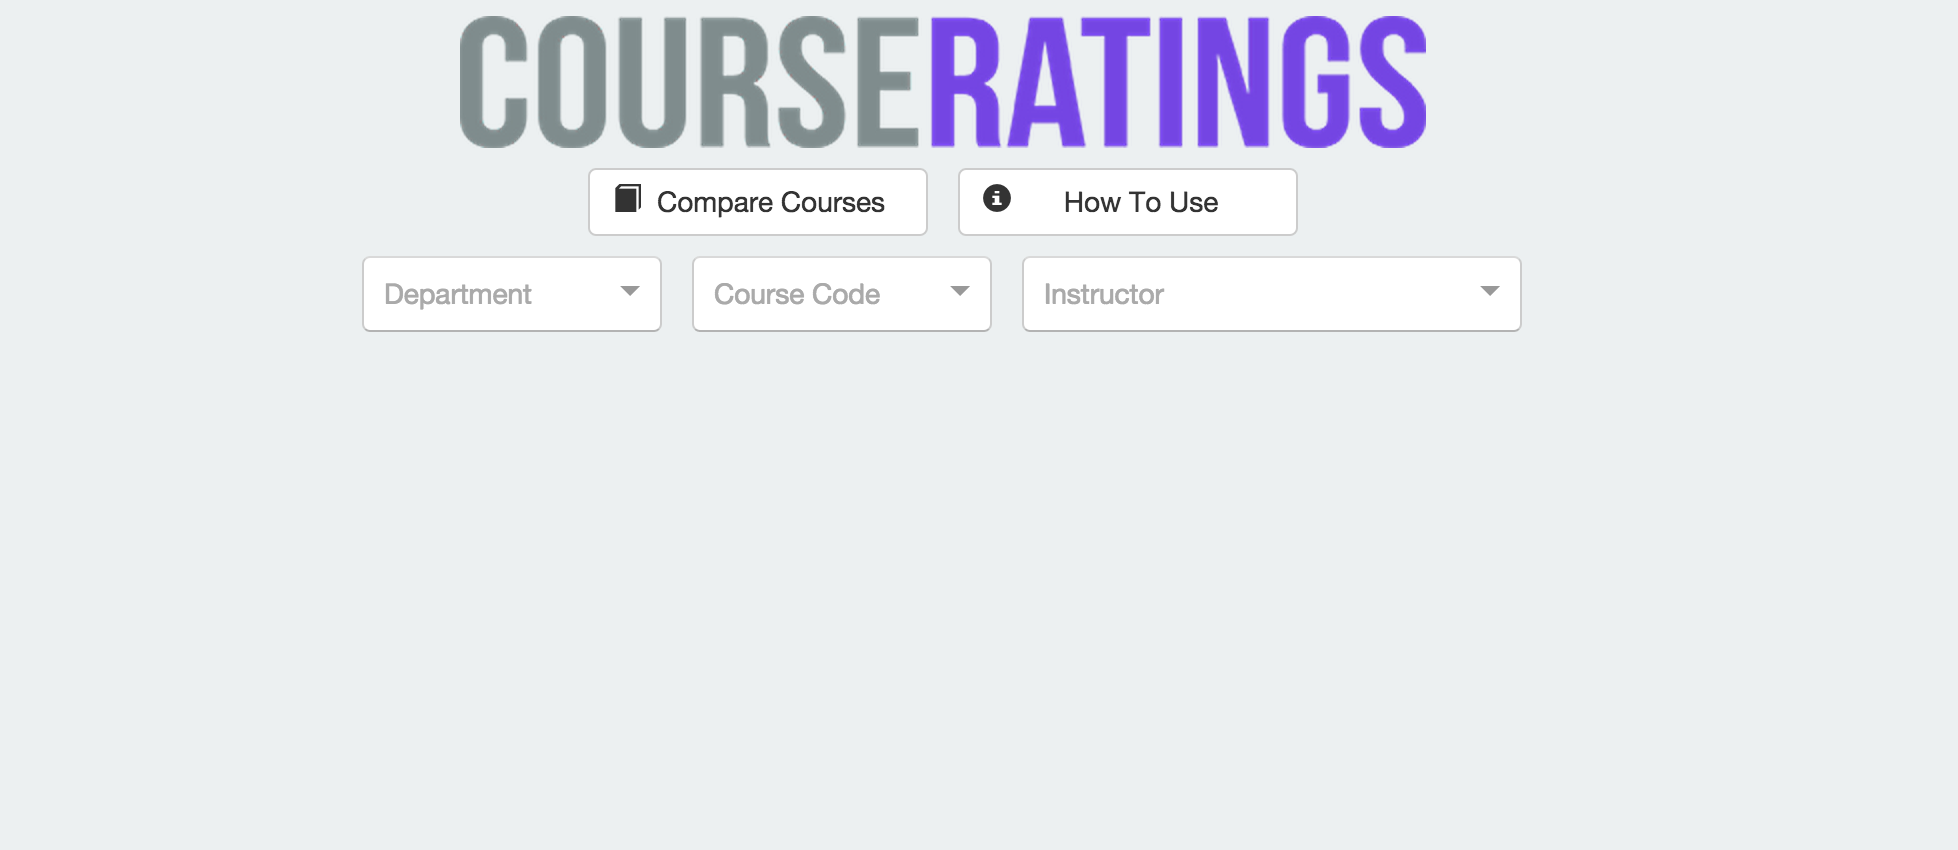
\includegraphics[width=\columnwidth]{figs/landingPage.png}
\vspace*{-0.25in}
\caption{CourseRatings landing page with the 3 search boxes.}
\label{fig:landing}
\end{center}
\end{figure}

Once CourseRatings has loaded, the user is presented with a logo, two buttons, and three drop down boxes on an otherwise empty page (see Figure \ref{fig:landing}). We decided to leave the page empty to let the users focus on the controls. The first button, ``Compare Courses'', loads the course comparison page. The second button, ``How To Use'', loads the tutorial page. This tutorial provides a brief overview of how to use CourseRatings and all of the features that users can take advantage of. The three drop down boxes allow a user to specify a department, course code, and/or instructor. CourseRatings returns the intersection of the specified search fields. After one or more search boxes are filled out, a table summarizing the search results appear (see Figure \ref{fig:searchResults}).

\begin{figure}[t]
\begin{center}
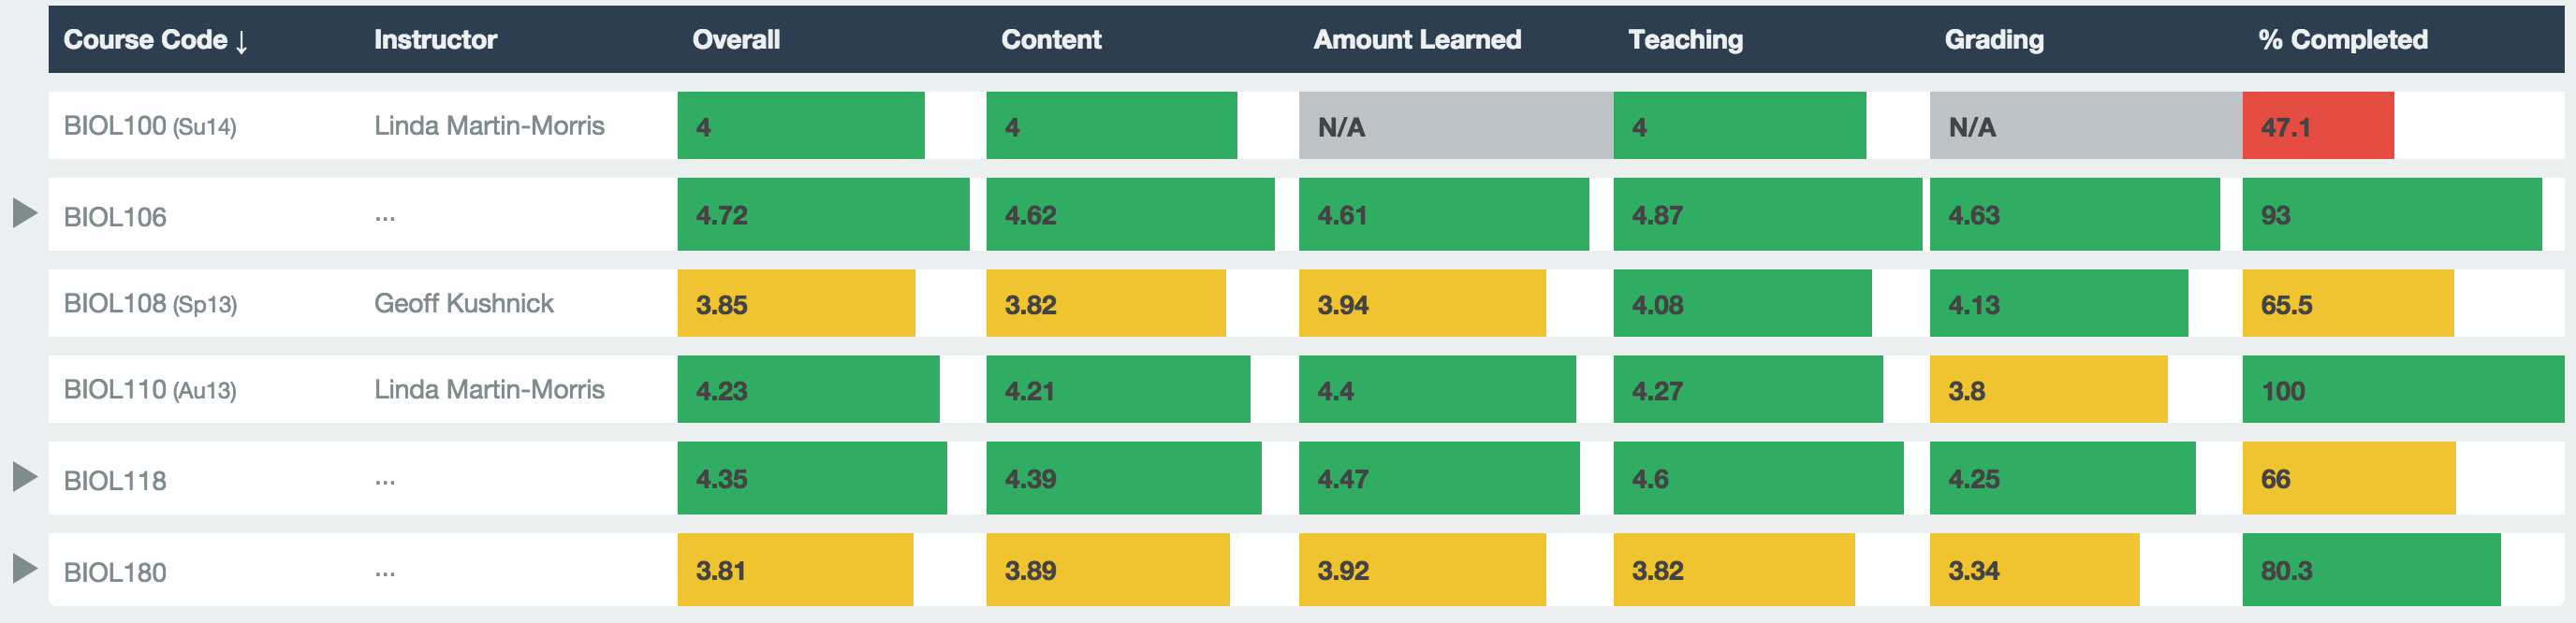
\includegraphics[width=\columnwidth]{figs/searchResults.png}
\vspace*{-0.25in}
\caption{Search results for all 100 level classes in the BIOL dep.}
\label{fig:searchResults}
\end{center}
\end{figure}

\subsection{Exploring Courses}
The search results table displays a course or instructor per row (depending on the search criteria). It rates each course or instructor along five dimensions - overall, content, amount learned, teaching and grading. It also displays the percentage of students in a class that have filled out the course evaluation survey. Clicking on a column name will sort the entries by that column -- a second click will reverse the sorting. An arrow to the right of the column name indicates if the column is in ascending or descending order. Some rows in the table may have a triangle next to them, indicating that there have been multiple offerings of that course. Clicking on the triangle will expand the row to show all offerings of the class and clicking on the triangle again will collapse the rows.  Expanded rows sharing the same course code/instructor and time are different sections taught during the same quarter.

Hovering over an entry in the ``\% Completed'' column will show the number of students who filled out evaluations for that class as a fraction. Hovering over all other column entries will show the average department score for that column. The entries in the table use three encodings to indicate whether the rating is good. Each rating is colored green (if it is good), yellow (if it is adequate), or red (if it is poor). The length of the shaded region also varies depending on the rating (with better ratings having longer lengths). This allows users to quickly get a big picture view of the quality of the courses or instructors returned by the search query.

Depending on how many search boxes are filled out, one of three pages will load. These pages are similar, with a few important differences that dictate what is shown to the user.


\subsubsection{Department Page}
If only the name of the department is specified with the two other search boxes empty, the department page will load. It shows all courses offered by the specified department in a table format described previously. The top 5 courses and instructors in this department are listed at the top of the page. These are computed with a linear combination of features in the data including overall rating and the number of entries for that course/instructor.

\subsubsection{Course Page}
If both the department name and course number are entered into the search, the course page will load. The course page displays the name and description of the selected course. It also lists all instructors who have taught the specified course. A line graph at the top shows the overall rating for each instructor during different quarters. A maximum of 5 instructors are shown on the graph. (see Figure \ref{fig:coursePage})

\subsubsection{Instructor Page}
If only the name of the instructor is specified, the instructor page will load.  This page is very similar to the course page.  The instructor page lists all courses taught by the specified instructor. A line graph at the top shows the overall rating for each of the courses taught by the instructor. A maximum of 5 courses are shown on the graph.

On both the course and instructor pages, the line graph displays the quarter on the X axis and the overall rating on the Y axis. Quarters for where there is no data point are left blank. Hovering over each dot displays its overall rating for easy access to the underlying data.

Clicking on a course code or instructor name in the table on any page will take you to the corresponding course page or instructor page respectively.

\begin{figure}[t]
\begin{center}
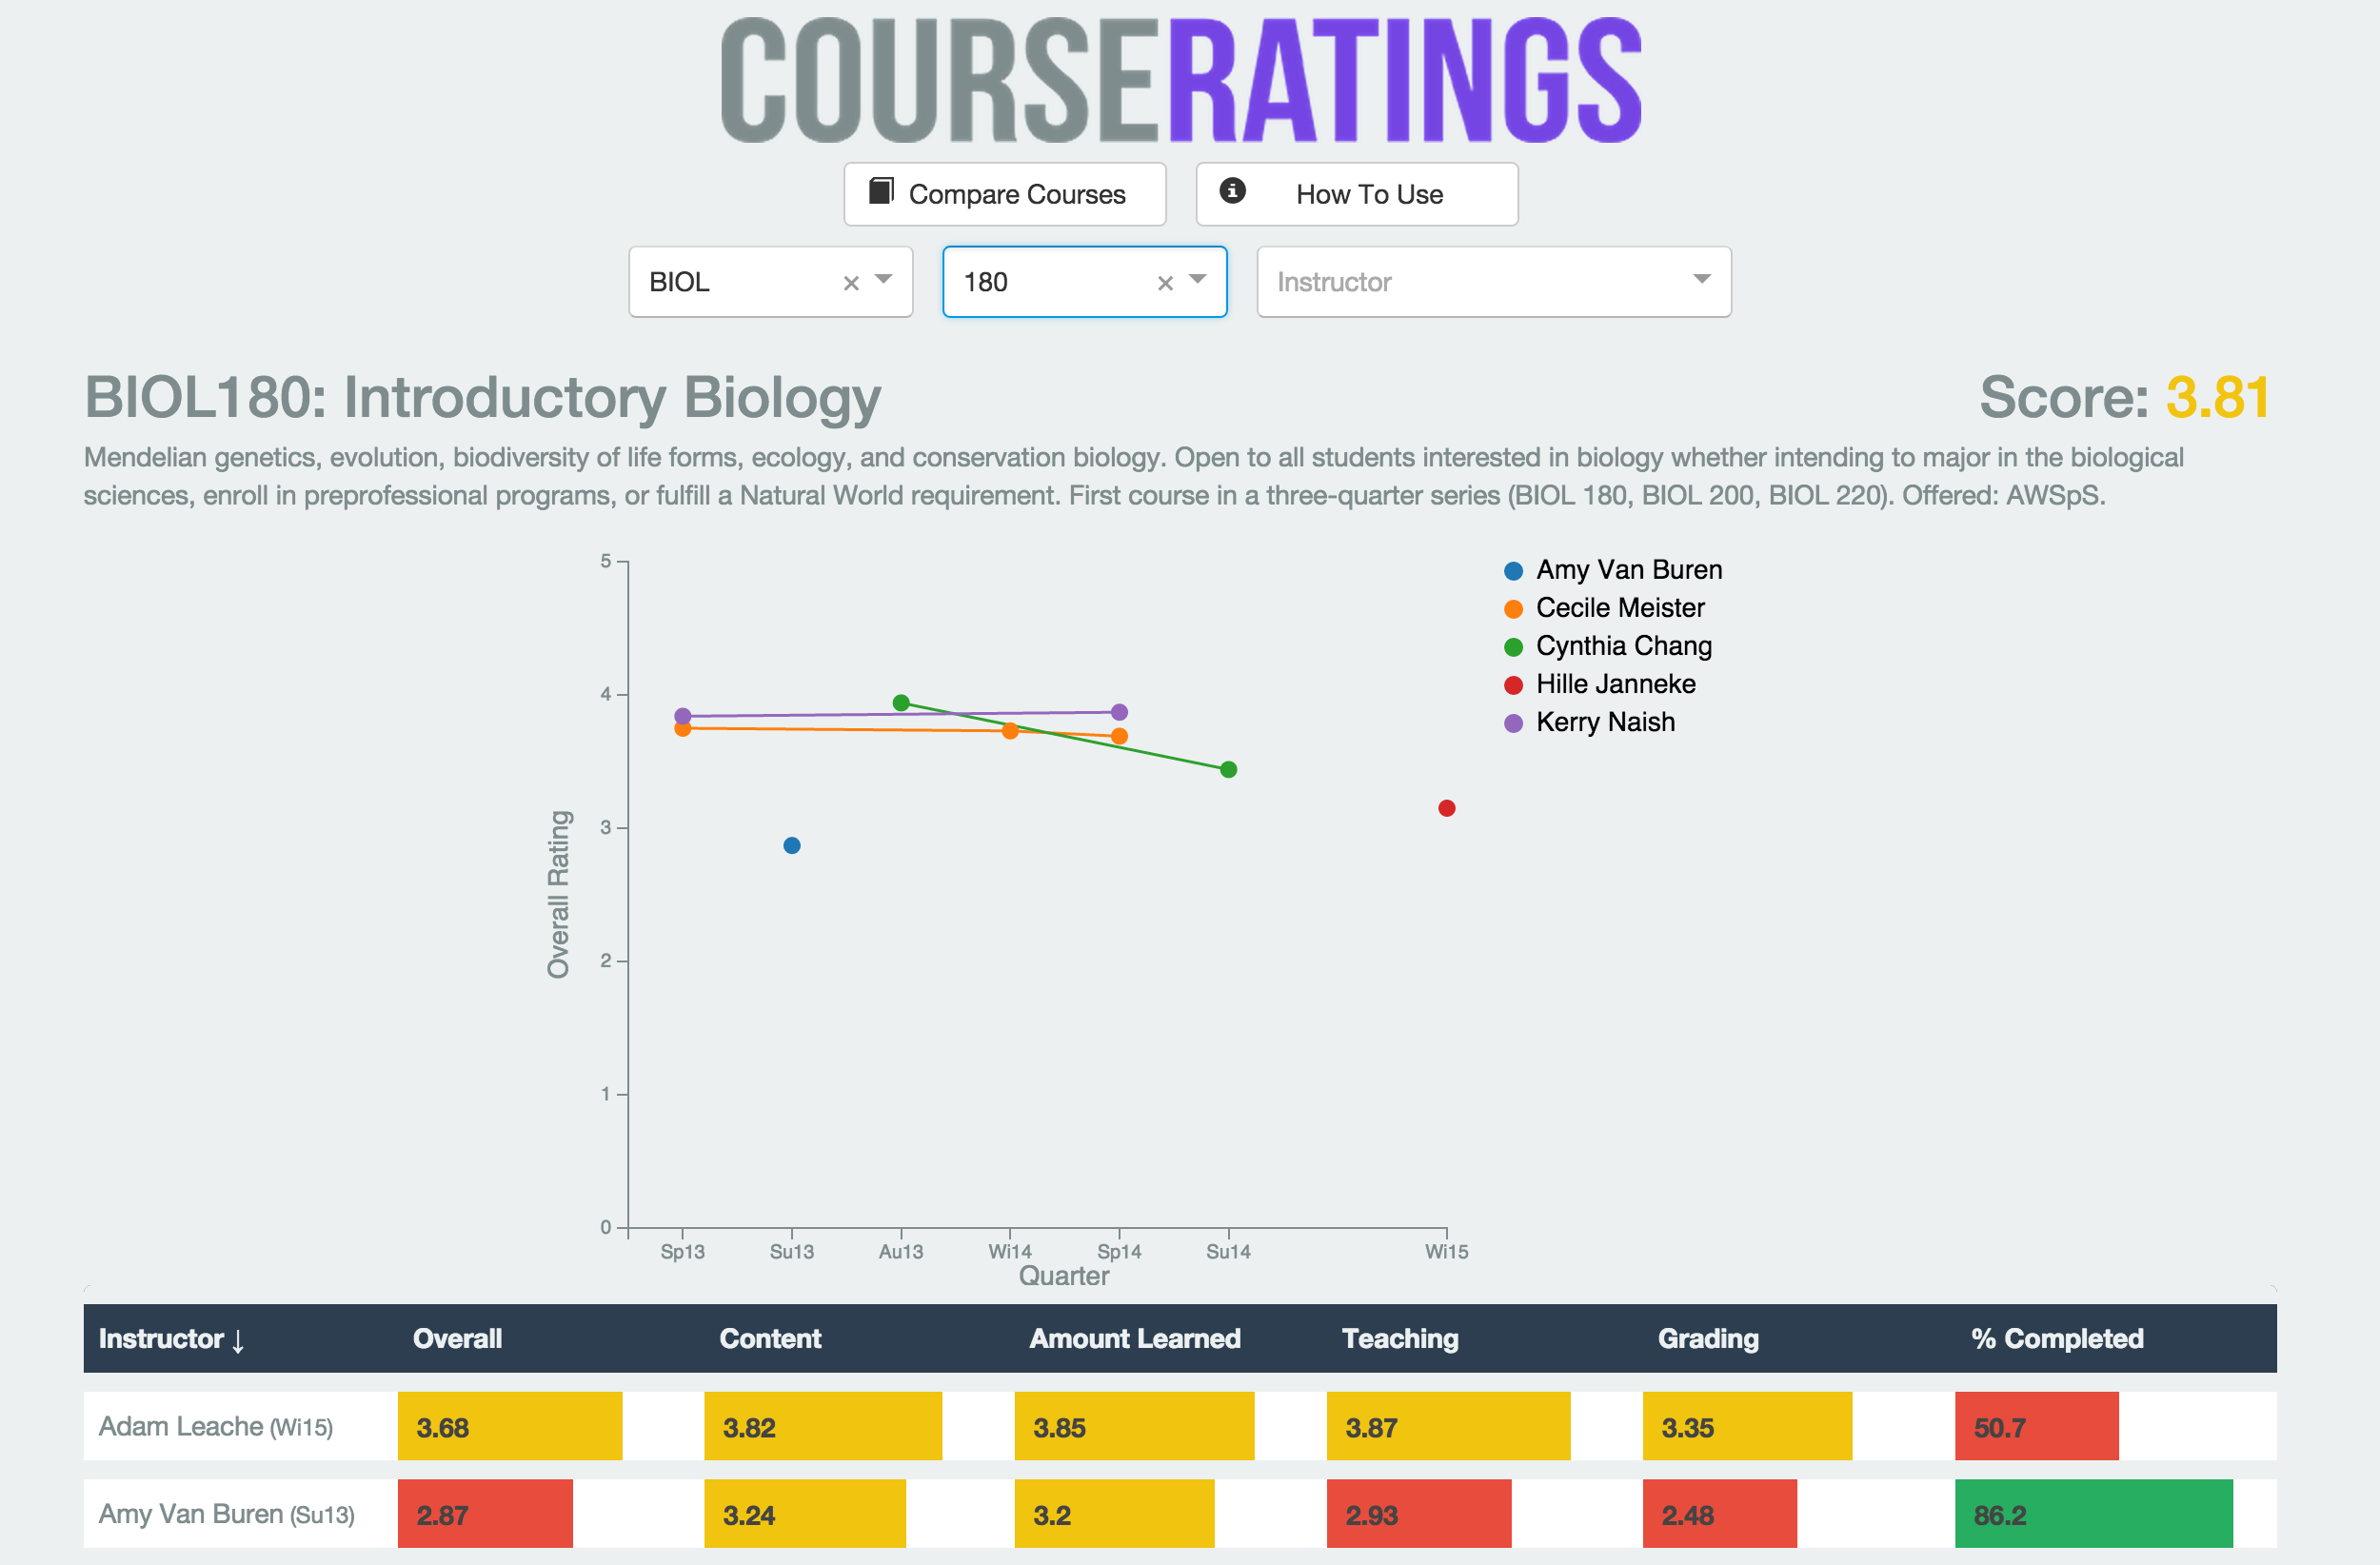
\includegraphics[width=\columnwidth]{figs/coursePage.png}
\vspace*{-0.25in}
\caption{An example of what the course page looks like for BIOL 180.}
\label{fig:coursePage}
\end{center}
\end{figure}

\subsection{Comparing Courses}
Clicking on the ``Compare Courses'' button at the top of the page takes the user to the course comparison page. It contains two drop down boxes. The first allows the user to specify a department, and the second a course code. After the user specifies a department and course code, a table summarizing the rating of the course will appear (see Figure 4).

\begin{figure}[t]
\begin{center}
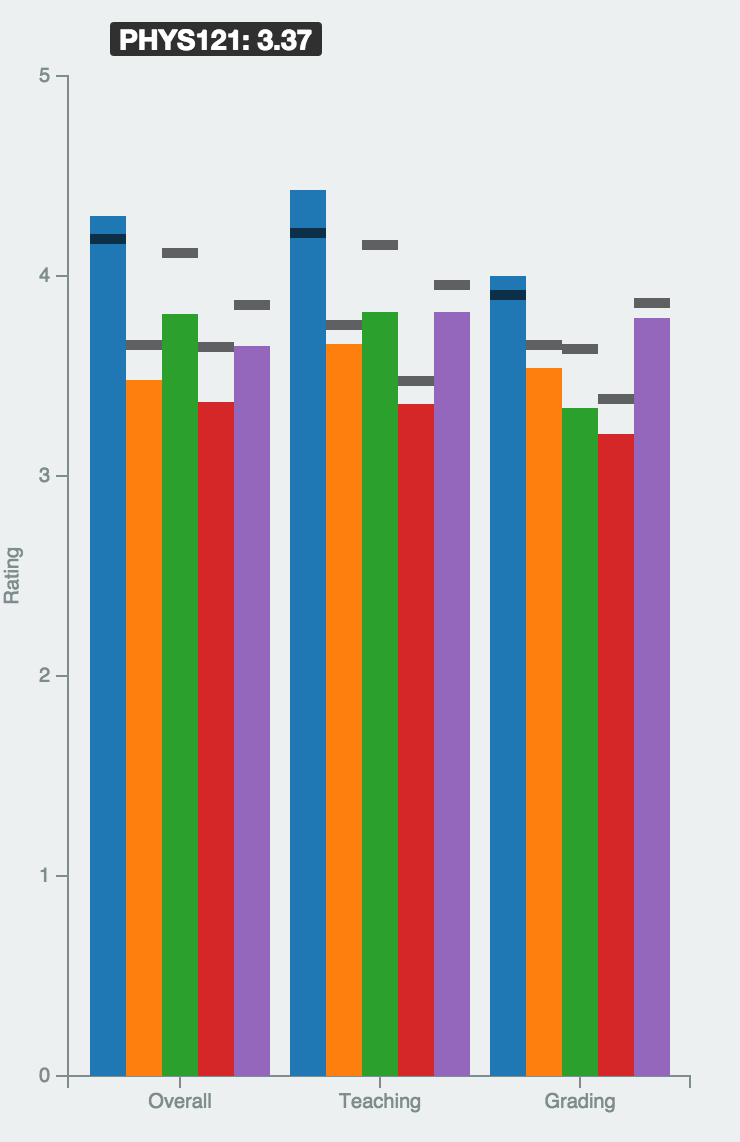
\includegraphics[width=0.55\columnwidth]{figs/barChart.png}
\vspace*{-0.1in}
\caption{Comparison of the intro sciences.}
\label{fig:coursePage}
\end{center}
\end{figure}

The + and - buttons on either side of the drop down boxes can be used to increase and decrease the number of courses being compared respectively. The + button adds another set of drop down boxes, while the - button removes a set of drop down boxes. These drop down boxes can be used to specify more courses.

Hovering over a bar will display the name of the course represented by the bar, as well as its value. It will also display a black horizontal bar indicating the average rating of classes in that department. For example, in figure 4, the cursor is hovering over the bar representing CSE 142. The black line indicates the average amount learned rating in the CSE department. More information on what each bar represents can be found in the legend next to the chart.

When a new course is specified, or an existing course is removed or modified, the table and chart update automatically. The course, instructor, department, tutorial and comparison pages all load instantaneously, with the tables and charts rendered quickly. However, the initial page takes several seconds to load upon start up, which is when a loading GIF is displayed.

\section{Discussion}

We spoke to many people about CourseRatings as well as UW's CEC when prototyping, implementing, and presenting this application. Most people we spoke to had used the Course Evaluation Catalog before. Every single one of these people - both students and instructors - found it an unpleasant experience. One person remarked that the design hadn't changed in over a decade from when they were a student.

Additionally, there was a lot of interest in our website, and we received many requests to make it public.\footnote{\href{students.washington.edu/drapeau/course_ratings/}{students.washington.edu/drapeau/course\_ratings/}} Before the poster session, we integrated Google Analytics\footnote{\href{www.google.com/analytics}{www.google.com/analytics}} onto our site in order to track the growth after the presentation. Since presenting on Monday, we have had 121 sessions with 58 unique users. The average duration these people spent on the site was slightly longer than 11 minutes.

\subsection{Insight}
Many students remarked that they would be using the site in the future to decide which courses to take. One student mentioned that he was required to take an introductory science class (either Biology, Physics or Chemistry), and was going to use CourseRatings' comparison page to decide which class to take. Another student used the course information page to to choose which instructor she wanted to take a particular class from. Still others used the search function to browse departments and classes to spot interesting trends. For example, one student wanted to learn about the best and worst 400 level classes in the Computer Science \& Engineering department. Another student wanted to see if some departments had more “green” ratings than others. Thus, CourseRatings functions as a visualization tool, allowing students to compare instructors and courses. It also allows students to spot larger trends in departments. These types of interactions would be impossible with UW's Course Evaluation Catalog. Discovering trends or comparing courses/instructors using this catalog requires clicking on multiple links and attempting to summarize the ratings of a particular course offering, and then comparing these ratings to those of another course offering.

Many of the instructors that tried CourseRatings out used it to search for their own instructor pages. Some of them discovered that, to their surprise, some of their courses were rated significantly higher than others. Others compared the ratings of a class they taught to ratings of the same class taught by different instructors and tried to figure out what about each instructor's teaching style led to the ratings of each class. These types of observations would be impossible with UW's Course Evaluation Catalog, which neither stores data for multiple quarters nor allows for easy comparison. Thus, CourseRatings allows instructors to learn about what students think about their teaching styles, as well as compare their teaching styles to those of instructors whose teaching styles they are familiar with. It also allows them to see whether their teaching style needs to be adapted for certain courses.

\vspace{-5 pt}
\subsection{Improvement}
One of the suggestions we received was to only display the course code drop down box if the department drop down box was filled, because searching for a course code alone in CourseRatings isn't very useful. Accordingly, we updated CourseRatings to have the course code drop down box be grayed out unless a department is specified.

Another suggestion we received was to explain the meaning and significance of the data displayed in CourseRatings' tutorial. Students that haven't filled out a course evaluation survey before could be confused about what each dimension indicates, or where we get our data from. As a result, we updated our tutorial to explain where we get our data from, as well as what that data means, at the very beginning.

As discussed in earlier sections, we created bar charts that allowed students to compare courses along five dimensions - overall, content, amount learned, teaching, and grading. However, one piece of feedback we received was that the number of bars made it difficult to quickly compare classes. Additionally, there is likely correlation between some of the dimensions (for example, content and amount learned are likely to be similar). Since the information in the bar chart is also present in the table displayed below it, it was suggested that we reduce the number of dimensions in the bar chart to make it less cluttered. Accordingly, we picked updated the bar chart to display the following three dimensions - overall, teaching and grading.

One drawback of our current design is that users cannot use the back button to go back to a previous search. We mitigated this by providing buttons that users could click on to navigate between exploring courses, comparing courses, and viewing the tutorial. Clicking on course numbers and instructor names, as well as deselecting fields in the drop down boxes also allow for efficient navigation. However, many users still used the back button - perhaps out of habit. As a quick fix, users are now warned once the back button is pressed that they are leaving the page. Ensuring that the back button works would make our website even more intuitive to use.

\vspace*{-5 pt}
\section{Future Work}
Additionally, we would like to improve our integration with the University of Washington Time Schedule, which lists all the courses offered in the current or upcoming quarter. One frequently requested feature is displaying which courses are being currently offered, or offered next quarter. Deciding on a class to take, only to discover that it is not being offered for another year, is likely an unpleasant experience. We hope that allowing users to restrict search results to courses being offered in the current or next quarter will prevent such experiences from happening. This can be done by scraping UW’s Time Scheduling, and storing when a course is going to be offered.

Finally, we want to keep scraping the Course Evaluation Catalog to gather more data on courses offered in the future. This would require scraping data regularly, as well as updating the scraper when the format of the Course Evaluation Catalog changes, which is unlikely. As mentioned earlier, the course catalog only contains information for the past two or three quarters. However, we have been scraping data for over a year now, and have data spanning eight quarters. Students and instructors alike have found our visualizations useful, despite the fact that we have only had eight quarters worth of data. With more data, we hope to be able to provide users with even more insight into courses and instructors.

\vspace*{-5 pt}
\section{Conclusion}
This paper presents CourseRatings, an online tool to visualize the ratings of courses at the University of Washington. Built as an alternative to UW’s Course Evaluation Catalog, CourseRatings is built around three core features: search, table visualizations, and trend visualizations. CourseRatings allow users to view ratings on courses and instructors, as well as visualizations on how they have changed over time. Users can search for, sort through, expand on and learn more about these ratings. CourseRatings also allows users to compare courses against each other on three dimensions - Overall, Teaching and Grading. This tool solves the four major problems of the Course Evaluation Catalog -- the inability to search for classes or instructors, the difficulty of understanding what the given ratings say about a class, the difficulty of comparing classes, and the lack of features that allow users to see trends. It is our hope that CourseRatings makes it easier for students to register for classes and for instructors to better understand the feedback they receive.

% \section{Acknowledgments}

% We thank Daniel Gorrie, Aaron Nech, and anyone who provided feedback for discussions. We also thank Jeff Heer, Jeff Snyder, and Dominik Moritz for feedback and insights.
\vspace*{-5 pt}
\bibliographystyle{abbrv}
\bibliography{references}

\end{document}
